\section{Output Analysis}
\subsection{Correlation analysis}
We have not been able to create correlograms.
Correlation analysis by creating correlograms and looking at statistics and (the absence of) repetitive patterns to determine that replications were uncorrelated failed.
Therefore, we do not know if our replications are properly uncorrelated.
 
We did take other measures to limit the possibilities of correlation.
Between each of the replications, the system and statistics were (re)initialized.
This is not enough, indicated by the Arena generated .out file, which contains a large number of ``(Insuf)" fields for the half-widths in stead of accurate values.
In addition, also several ``(Corr)" fields can be found in the file.
It is uncertain if our replications are properly uncorrelated.

The point of correlation analysis is to find the right number of replications to simulate with.
As we have not found a proper number by doing the usual correlation analysis, the simulation results may be affected.
This is worth considering when reviewing the validity of the results.

\subsection{Sensitivity analysis}
\subsubsection{Number of cashiers}
We investigate the influence of the number of cashiers on three metrics, the average car throughput time, the average truck throughput time and the block rate.
\autoref{fig:fewercashiers} shows the development of these metrics over 5 scenarios.
The y-axis reads a percentage for the block rate and hours for the throughput times.

\begin{figure}[ht!]
	\centering
	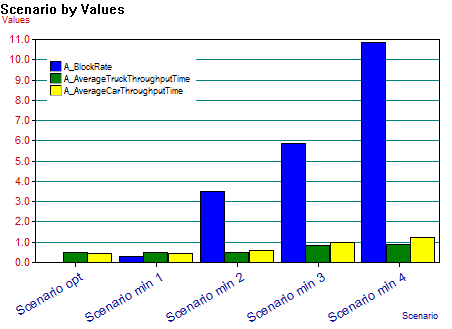
\includegraphics[width=.75\textwidth]{images/fewerCashiers.png}
	\caption{Throughput times and block rates in the optimal solution and cases with 1,2,3 and 4 cashiers less.}
	\label{fig:fewercashiers}
\end{figure}

We see that the block rate is most influenced by decreasing the number of cashiers.
Furthermore, it can be seen that one cashier less still results in a legal solution, indicating that our optimal solution is not in fact optimal.


\subsubsection{Future scenario}
It is expected that the number of customers as well as the amount of fuel they buy will decrease in the future.
This is due to the rising popularity of electric vehicles as well as the increasing fuel efficiency of vehicles.
In this scenario, we investigate how the cashier schedule should be altered when both the arrival rate and the bought fuel amounts decrease.
We have investigated three cases, with decreases of 10, 20 and 30\% of arrivals and amounts.
For each case, we have performed 1000 simulations and 1 replication per simulation.

The number of shifts decreases drastically when the demand decreases.
The optimal solution in the standard case yielded 22 shifts.
When the demand decreases with 10\%, the number of shifts is 17.
Demand decreases of 20 and 30\% yield 16 and 15 shifts respectively.